
\chapter[Precision Optimisation of Data-paths]{Precision Optimisation of Data-paths}

\label{ch:precision}

%%%%%%%%%%%%%%%%%%%%%%%%%%%%%%%%%%%%%%%%%%%%%%%%%%%%%%%%%%%%%%%%%%%%%%%%%%%%%%%%%%%%%%%%%%%%%%%%%%%%%%%%%%%%%%%%%%%%%%%%%%%%%%%%%%%%%%%%%%%%%%%%
\section{Introduction}
\label{sec:precision_intro}

This chapter presents a precision optimisation approach to maximise real-time performance of reconfigurable systems.
The proposed approach is applied to image-guidance of medical surgery robot.

\gls{pq} is an important compute-intensive and real-time application which requires substantial acceleration before it can be used in clinical setting.
It is because fast and efficient \gls{pq} (update frequency above 1~kHz) is required to maintain smooth and steady manipulation guidance which is particularly essential for soft tissue surgery having large-scale and rapid tissue deformations.
This real-time requirement, as well as the intrinsic complexity of the algorithm, make \gls{pq} computationally challenging as a high update frequency above 1~kHz is required. 
The computation burden is increased by the need to model the shape of tissue and surgery robot by more than~1~million~points.

Due to its compute-intensive nature, \gls{pq} can greatly benefit from hardware acceleration.
However, the massive amount of floating-point computations constitute a long data-path which is resource-demanding.
Even if we could implement the data-path in an \gls{fpga}, the acceleration would be restricted by low parallelism and clock frequency.
This challenge limits the implementation of \gls{pq} on an \gls{fpga}.

In this chapter, we derive a \gls{pq} formulation which allows objects to be represented in complex geometry with points.
To leverage the advantages of \gls{fpga}s, function transformation eliminates iterative trigonometric functions such that the algorithm can be fully-pipelined.
We increase data-path parallelism by adopting a reduced precision data format which consumes fewer logic resources than high precision.
To maintain the accuracy of results, potential incorrect outputs are re-computed in high precision.
We design a novel memory architecture for buffering potential outputs and maintaining streaming data-flow.
We further exploit the run-time reconfigurability of \gls{fpga} to optimise precision dynamically.
To the best of our knowledge, our work is the first to apply reconfigurable technology to narrow-phase \gls{pq} computation.

The contributions of this chapter are as follows.
\begin{itemize}
\item A hardware-friendly \gls{pq} formulation for calculating the relative placement of objects modelled by points with complex morphology, which facilitates
restructuring of trigonometric and search-functions to be amenable to parallel implementation in hardware.
\item Enhanced parallelism by treating input points as a novel data structure propagating through pipelines, 
together with \gls{fpga}-specific optimisations such as adapting \gls{pq} to reduced precision arithmetic,
supporting multiple precisions in a novel memory architecture, and automating precision management with run-time reconfiguration.
\item Implementation in a reconfigurable platform with four \gls{fpga}s which is shown to be 478 times faster than a single-core \gls{cpu}, 58 times faster than a 12-core \gls{cpu} system, 9 times faster than a \gls{gpu}, and 3 times faster than a 4-\gls{fpga} system implemented in double precision.
\end{itemize}

The rest of the chapter is organised as follows.
Section~\ref{sec:precision_formulation} presents our proposed \gls{pq} formulation.
Section~\ref{sec:precision_optimisation} discusses the optimisation of \gls{pq} for reconfigurable system.
Section~\ref{sec:precision_implementation} describes the system design that maps \gls{pq} to a reconfigurable system.
Section~\ref{sec:precision_evaluation} provides experimental results and
Section~\ref{sec:precision_summary} concludes our work.

%%%%%%%%%%%%%%%%%%%%%%%%%%%%%%%%%%%%%%%%%%%%%%%%%%%%%%%%%%%%%%%%%%%%%%%%%%%%%%%%%%%%%%%%%%%%%%%%%%%%%%%%%%%%%%%%%%%%%%%%%%%%%%%%%%%%%%%%%%%%%%%%
\section{Formulation of PQ}
\label{sec:precision_formulation}

In this section, we derive our modified \gls{pq} process which was originally proposed in~\cite{kwok13}. 
The significance of this modification is to formulate the \gls{pq} capable of processing the contours in complex shapes. 
As shown in Figure~\ref{fig:pqa_ch3}, \gls{pq} allows the analytical measure of the shortest Euclidean distance between an arbitrary set of points and a series of segments $\Omega_j$ (cf. Definition 1) which has been a well-known representation of a complex three-dimensional object~\cite{ponce89}. 
Each segment $\Omega_j$ is enclosed by two adjacent contours which are outlined by points arranged in polar coordinates; 
hence, it outperforms the existing narrow-phase \gls{pq}s which are only compatible with convex objects.

\begin{mydef}
Each contour is denoted by $C_j$, $\forall j \in [1,...,N_C]$.
A single segment $\Omega_j$ comprises two adjacent contours $C_j$ and $C_{j+1}$.
$P_j$ is the centre of the contour $C_j$.
$M_j$ is the tangent of centre line of contour $C_j$.
$^j\omega_i=[^j\omega_{xi},^j\omega_{yi},^j\omega_{zi}]^T, (i=1,...,W)$ are the contour points,
where $W$ is the number of points outlining each contour.
\end{mydef}

Four steps are taken to calculate the point-to-segment distance $\delta_j$, which is shown in Figure~\ref{fig:pqa_ch3} as the shortest distance $\delta_j$ between a point $\boldsymbol{x}$ and the corresponding edge $^jV_2 \rightarrow ^jV_3$.
%the formulation is modified to efficiently find out the four-edge polygon which is a cross section cutting through the poles of the two contours as well as the 3D point. 
%The \gls{pq} is proceeded effectively to calculate the shortest distance only between a point and the corresponding edge of the polygon. 
%Vertices ${^jV}_3$ and ${^jV}_4$ are then to be calculated as the linear combination of, respectively, ${^{j-1}\omega_i}$ and ${^{j-1}\omega_{i+1}}$, and ${^{j}\omega_i}$ and ${^{j}\omega_{i+1}}$.
%\noindent \textbf{Pre-processing step}:
%This step is done at design time.
Before introducing these steps, we describe the computation using polar coordinates.
Given a contour $C_j$, $^j\phi_i$ is the polar angle corresponding to contour points $^j\omega_i$.
The polar angles of all the $^j\omega_i$ along the contour, i.e. $^j\omega_1, ..., ^j\omega_W$, have to be computed. 
This computation can be further simplified by ignoring an axis coordinate. 
The poles and the contour points are then projected either on X-Y, Y-Z or X-Z plane based on the following conditions:   

\begin{equation}
\begin{aligned}
\mbox{if } &|M_{zj}| = \max \left ( {|M_{xj}|,|M_{yj}|,|M_{zj}|} \right ) \mbox{, } \\
&{^j\omega}^{\prime}_i = [{^j\omega}_{1i},{^j\omega}_{2i}]^T = [{^j\omega}_{xi},{^j\omega}_{yi}]^T, P^{\prime}_j=[P_{xj},P_{yj}]^T \mbox{, } \\
\mbox{if } &|M_{xj}| = \max \left ( {|M_{xj}|,|M_{yj}|,|M_{zj}|} \right ) \mbox{, } \\
&{^j\omega}^{\prime}_i = [{^j\omega}_{1i},{^j\omega}_{2i}]^T = [{^j\omega}_{yi},{^j\omega}_{zi}]^T, P^{\prime}_j=[P_{yj},P_{zj}]^T \mbox{, } \\
\mbox{if } &|M_{yj}| = \max \left ( {|M_{xj}|,|M_{yj}|,|M_{zj}|} \right ) \mbox{, } \\
&{^j\omega}^{\prime}_i = [{^j\omega}_{1i},{^j\omega}_{2i}]^T = [{^j\omega}_{zi},{^j\omega}_{xi}]^T, P^{\prime}_j=[P_{zj},P_{xj}]^T \mbox{, } 
\end{aligned}
\label{eqt:preprocess1}
\end{equation}

where $M_j=(M_{xj}, M_{yj}, M_{zj})$ is the tangent of centre line of contour $C_j$.

\begin{figure}[ht]
\begin{center}
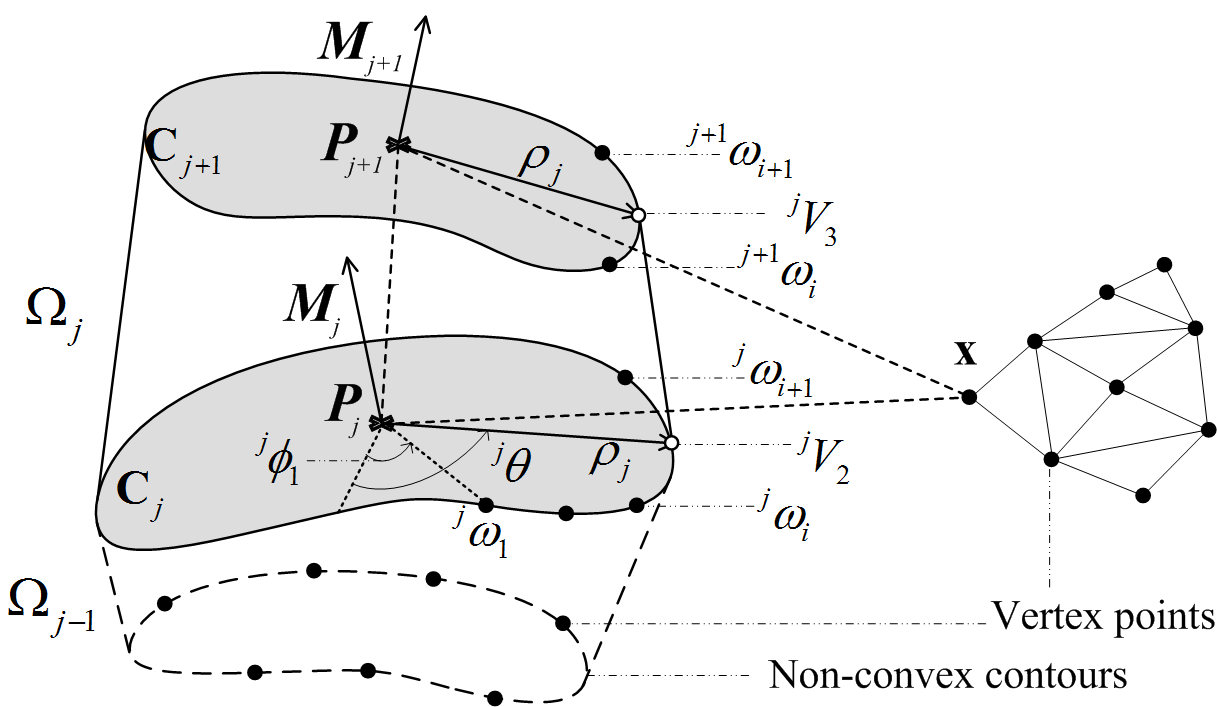
\includegraphics[width=0.7\textwidth]{3_precision/figures/pqa}
\end{center}
\caption[Various sets of points aligned on a series of contours; A set of points located on an arbitrary form of mesh.]{(Left) Various sets of points aligned on a series of contours; 
(Right) A set of points located on an arbitrary form of mesh.}
\label{fig:pqa_ch3}
\end{figure}

Then ${^j\phi_i}$ is calculated as follows:

\begin{equation}
\begin{aligned}
\overline{{^j\omega}^{\prime}_i} = {^j\omega}^{\prime}_i - P^{\prime}_j \mbox{ , } \qquad
{^j\phi}_i = atan2 \left ( \overline{{^j\omega}_{2i}},\overline{{^j\omega}_{1i}} \right ) \mbox{.}
\end{aligned}
\label{eqt:preprocess2}
\end{equation}

We will explain the details of $atan2$ is Section~\ref{sec:precision_trigo}.

\noindent \textbf{Step 1}:
Find the normal of a plane containing three points: $\boldsymbol{x}$, $P_j$ and $P_{j+1}$.
The symbol $\times$ denotes a cross product of two vectors in three-dimensional space.
The normal $n_j$ is calculated by:

\begin{equation}
\begin{aligned}
n_j = \left ( P_j-x \right ) \times \left ( P_{j+1}-x \right ) \mbox{.}
\end{aligned}
\label{eqt:normal}
\end{equation}

\noindent \textbf{Step 2}:
Calculate vectors $\rho_j$ and $\rho_{j+1}$ which are respectively perpendicular to tangents $M_j$ and $M_{j+1}$ and are both parallel to the plane with normal $n_j$.

\begin{equation}
\begin{aligned}[c]
\rho_j = n_j \times M_j
\end{aligned}
\mbox{ , }
\qquad
\begin{aligned}[c]
\rho_{j+1} = n_j \times M_{j+1} \mbox{.}
\end{aligned}
\label{eqt:rho}
\end{equation}

\noindent \textbf{Step 3}:
Determine a 4-vertex polygon outlined by \mbox{${^jV}_{i=1...4}\in \Re^{3 \times 1}$} which is a part of the cross-section of segment $\Omega_j$.
This section is cut by a plane containing the point $\boldsymbol{x}$ and the line segment $P_j \rightarrow P_{j+1}$.

\begin{equation}
\begin{aligned}[c]
{^jV}_1 &= P_j \mbox{,} \\
{^jV}_4 &= P_{j+1} \mbox{,}
\end{aligned}
\qquad
\begin{aligned}[c]
{^jV}_2 &= P_j + t_j \cdot \rho_j \mbox{,} \\
{^jV}_3 &= P_{j+1} + t_{j+1} \cdot\rho_{j+1} \mbox{.}
\end{aligned}
\label{eqt:vertices}
\end{equation}

At this stage, we need to calculate $t_j$ and $t_{j+1}$ of Equation~\ref{eqt:vertices}.
This can be achieved by mapping the values of $\rho_j$ to a two-dimensional plane.
The two-dimensional mapping of $\rho_j$ is $\rho^{\prime}_j$.

\begin{equation}
\begin{aligned}
\mbox{if } &|M_{zj}| = \max \left ( {|M_{xj}|,|M_{yj}|,|M_{zj}|} \right ) \\
&\rho^{\prime}_j = [\rho_{1j},\rho_{2j}]^T = [\rho_{xj},\rho_{yj}]^T \mbox{,} \\
\mbox{if } &|M_{xj}| = \max \left ( {|M_{xj}|,|M_{yj}|,|M_{zj}|} \right ) \\
&\rho^{\prime}_j = [\rho_{1j},\rho_{2j}]^T = [\rho_{yj},\rho_{zj}]^T \mbox{,} \\
\mbox{if } &|M_{yj}| = \max \left ( {|M_{xj}|,|M_{yj}|,|M_{zj}|} \right ) \\
&\rho^{\prime}_j = [\rho_{1j},\rho_{2j}]^T = [\rho_{zj},\rho_{xj}]^T \mbox{.}
\end{aligned}
\label{eqt:rhoprocess}
\end{equation}

Then we calculate ${^j\theta}$, the corresponding polar angle of $\rho^{\prime}_j$ by Equation~\ref{eqt:theta}.

\begin{equation}
\begin{aligned}
{^j\theta} = atan2 \left ( \rho_{2j},\rho_{1j} \right ) \mbox{.}
\end{aligned}
\label{eqt:theta}
\end{equation}

%Algorithm~\ref{algo:search} is performed to find ${^j\phi}$ and ${^{j+1}\phi}$ which embrace ${^j\theta}$.
A search is performed to find ${^j\phi_i}$ and ${^j\phi_{i+1}}$ such that ${^j\phi_i} \leq {^j\theta} \leq {^j\phi_{i+1}}$.
The polar angles $^j\phi_i$ and ${^j\phi_{i+1}}$ are calculated from Equation~\ref{eqt:preprocess2}.

%\begin{algorithm}
%\caption{Search ${^j\phi}$ and ${^{j+1}\phi}$ that embrace ${^j\theta}$}
%\footnotesize
%\begin{algorithmic}[1]
%\STATE{i=0}
%\WHILE{$!({^j\phi}_i\le {^j\theta} \le{^j\phi}_{i+1})$} \label{algo:check}
%	\STATE {i++}
%\ENDWHILE
%\STATE{Return $i$}
%\end{algorithmic}
%\label{algo:search}
%\end{algorithm}

Based on the value $i$ obtained from the search, $t_j$, which is used in Equation~\ref{eqt:vertices}, is calculated.

\begin{equation}
\begin{aligned}
a &= [(P_j-{^j\omega}_i)({^j\omega}_{i+1}-{^j\omega}_i)][({^j\omega}_{i+1}-{^j\omega}_i)\rho] \mbox{,} \\
b &= [(P_j-{^j\omega}_i)\rho]\|{^j\omega}_{i+1}-{^j\omega}_i\|^2 \mbox{,} \\
c &= \|\rho\|^2\|{^j\omega}_{i+1}-{^j\omega}_i\|^2-\|({^j\omega}_{i+1}-{^j\omega}_i)\rho\|^2 \mbox{,} \\
t_j &= \frac{a-b}{c} \mbox{.}
\end{aligned}
\label{eqt:t}
\end{equation}

\noindent \textbf{Step 4}:
Define the shortest distance to be zero if the point $\boldsymbol{x}$ lies inside the polygon $^jV_{i=1...4}$ on the same plane.
Referring to~\cite{preparata85}, it can be determined by three variables $\lambda_{i=1,...,3}$ calculated as follows:

\begin{equation}
\begin{aligned}
\lambda_i &= n_j \cdot \psi_i, i={1,...,3} \\
\mbox{s.t. } \psi_i &= (^jV_i-\textbf{x}) \times (^jV_{i+1}-\textbf{x}) \mbox{.}
\end{aligned}
\label{eqt:lamda}
\end{equation}

Here $n_j$ denotes the normal defined in Equation~\ref{eqt:normal} and $\psi_i$ denotes the normal of the plane containing $^jV_{i=1...4}$.
For all $\lambda_{i=1,...,3} \ge 0$, the shortest distance $\delta_j$ from point $\boldsymbol{x}$ to the segment $\Omega_j$ is assigned to zero such that $\delta_j(\boldsymbol{x})=0$.
Otherwise $\delta_j(\boldsymbol{x})$ will be considered as the distance from the point $\boldsymbol{x}$ to the line segment $^jV_2 \rightarrow ^jV_3$.
Referring to~\cite{weisstein}, such a point-segment distance in three-dimensional space can be calculated as shown in Equation~\ref{eqt:distance}:

\begin{equation}
\begin{aligned}
^j\mu = \frac{(^jV_2-X)\cdot(^jV_3-^jV_2)}{||^jV_3-^jV_2||^2} \mbox{,} \\
\chi_j = (1-^j\mu)^jV_2 + ^j\mu^jV_3 \mbox{,} \\
\delta_{j}(\textbf{x}) = ||\textbf{x}-\chi_j|| \mbox{.}
\end{aligned}
\label{eqt:distance}
\end{equation}

In consideration of many points and segments, Equation~\ref{eqt:dev_min} generally expresses the deviation in distance from a single coordinate $x_i$ to a series of constraint segments ($\Omega_{1},...,\Omega_{N_C-1}$), where $i=1,...,N_P$, $N_P$ is the total number of points belong to the mesh model, $N_C-1$ is the number of segments involved in the calculation.

%If so, we can count the resultant shortest distance $d$ as zero, as shown in Equation~\ref{eqt:d_zero}.
%The vector $n_v$ and $d_i$ respectively denotes the normal of the plane containing $V_{i=1...4}$ %and the point along with vertex $i$ and $i+1$.

%\begin{equation}
%\begin{aligned}
%d_i &= (V_i-x) \times (V_{i+1}-x) \mbox{ where } i=1...3 \\
%\lambda_i = n_j \cdot d_i \\
%d = 0 \mbox{ for } \lambda_{i=1,...,3} \ge 0
%\end{aligned}
%\label{eqt:d}
%\end{equation}

%\noindent \textbf{Step 5}:
%All the segments $\Omega_j$ are integrated closely with each other along the pathway.
%The closest point is paired with $\boldsymbol{x}$ and lies on the segment boundary, which is always found on a line segment between vertices ${^jV}_2$ and ${^jV}_3$.
%If point $\boldsymbol{x}$ is out of the polygon, ${^ju} \in \Re$ have to be found from Equation~\ref{eqt:mu}.
%It is the parameter for linearly interpolating the line segment ${^jV}_2 \rightarrow {^jV}_3$ such that $x^\prime = (1-\mu^j)^jV^2+\mu^jV^j_3$,
%where $x^\prime$ is the perpendicular projection of $\boldsymbol{x}$ on that line segment.

%\begin{equation}
%\begin{aligned}
%{^j\mu} = - \frac{({^jV}_2-X)\cdot({^jV}_3-{^jV}_2)}{\|{^jV}_3-{^jV}_2\|^2}
%\end{aligned}
%\label{eqt:mu}
%\end{equation}

%\noindent \textbf{Step 6}:
%For point $x^\prime$ lying in-between ${^jV}_2$ and ${^jV}_3$ such that ${^j\mu} \in [0,1]$, 
%Equation~\ref{eqt:delta} obtains the point-to-line distance as the shortest one to segment $\Omega_j%$.

%\begin{equation}
%\begin{aligned}
%\chi_j = [(1-{^j\mu}){^jV}_2+{^j\mu} {^jV}_3] \\
%\delta_j(\boldsymbol{x}) = \|\boldsymbol{x}-\chi_j\|
%\end{aligned}
%\label{eqt:delta}
%\end{equation}

%For ${^j\mu}<0$, $\delta_j=\|\boldsymbol{x}-{^jV}_2\|$.
%Otherwise if ${^j\mu}>1$, then $\delta_j=\|\boldsymbol{x}-{^jV}_3\|$.

%The mesh is represented by a set of vertex points.
%Let the vertex coordinates be $\boldsymbol{x}_i$, $i=1,...,X$, where $X$ is the number of points.
%Equation~\ref{eqt:dev_min} calculates the deviation in distance from a single coordinate $%\boldsymbol{x}_i$ to the constraint segments ${\Omega_{m+1},...,\Omega_{m+\Delta m}}$,
%where $\Delta m$ is the number of segments involved in the calculation.

\begin{equation}
\begin{aligned}
{_i\delta}_{N_C-1} = \min \left ( \delta_{1}(\boldsymbol{x}_i),\delta_{2}(\boldsymbol{x}_i),...,\delta_{N_C-1}(\boldsymbol{x}_i) \right ) \mbox{.}
\end{aligned}
\label{eqt:dev_min}
\end{equation}

The point with the maximum deviation, also known as penetration depth, is obtained below:

\begin{equation}
\begin{aligned}
d^{N_C-1} = \max_{i=1,...,N_P} \left ( {_i\delta}_{N_C-1}(\boldsymbol{x}_i) \right ) \mbox{.}
\end{aligned}
\label{eqt:dev_max}
\end{equation}


%%%%%%%%%%%%%%%%%%%%%%%%%%%%%%%%%%%%%%%%%%%%%%%%%%%%%%%%%%%%%%%%%%%%%%%%%%%%%%%%%%%%%%%%%%%%%%%%%%%%%%%%%%%%%%%%%%%%%%%%%%%%%%%%%%%%%%%%%%%%%%%%
\section{Optimisation for Reconfigurable Hardware}
\label{sec:precision_optimisation}

The \gls{pq} formulation sketched in the previous section is not entirely hardware-friendly.
In this section we discuss several techniques allowing \gls{pq} to benefit from \gls{fpga} technology.

\subsection{Transformation of Trigonometric and Search Functions}
\label{sec:precision_trigo}
%Line~\ref{algo:check} of Algorithm~\ref{algo:search} checks whether ${^j\phi}_i \le {^j\theta}$.
The search process in step 3 of \gls{pq} (described in Section~\ref{sec:precision_formulation}) checks whether \linebreak ${^j\phi}_i \le {^j\theta}$.

\begin{equation}
\begin{aligned}
{^j\phi}_i = atan2 \left ( \overline{{^j\omega}_{2i}},\overline{{^j\omega}_{1i}} \right ) \mbox{, } \\
{^j\theta} = atan2 \left ( \rho_{2j},\rho_{1j} \right ) \mbox{.} \\
\end{aligned}
\label{eqt:check1}
\end{equation}

$atan2(a,b)$ is not a hardware-friendly operator.
It requires the calculation of $tan^{-1}(a,b)$ and then determines the appropriate quadrant of the computed angle based on the signs of $a$ and $b$.
$tan^{-1}(a,b)$ is resource and timing expensive~\cite{altera_megafunctions} and not available in many \gls{fpga} libraries, therefore, we transform Equation~\ref{eqt:check1} to another form as shown below:

\begin{equation}
\begin{aligned}
{^j\phi}_i &= tan^{-1} \left ( \frac{\overline{{^j\omega}_{2i}}}{\sqrt{\overline{{^j\omega}_{1i}}^2+\overline{{^j\omega}_{2i}}^2}+\overline{{^j\omega}_{1i}}} \right ) \mbox{, } \\
{^j\theta} &= tan^{-1} \left ( \frac{\rho_{2j}}{\sqrt{\rho_{1j}^2+\rho_{2j}^2}+\rho_{1j}} \right ) \mbox{.}
\end{aligned}
\label{eqt:check2}
\end{equation}

$atan2$ is transformed to $tan^{-1}$ which is then cancelled out on both sides.
As a result, the comparison becomes:

\begin{equation}
\begin{aligned}
\frac{\overline{{^j\omega}_{2i}}}{\sqrt{\overline{{^j\omega}_{1i}}^2+\overline{{^j\omega}_{2i}}^2}+\overline{{^j\omega}_{1i}}} &\le \frac{\rho_{2j}}{\sqrt{\rho_{1j}^2+\rho_{2j}^2}+\rho_{1j}} \mbox{.}
\end{aligned}
\label{eqt:check3}
\end{equation}

In this case, square root calculation is much easier to be mapped to hardware.

\subsection{Applying Reduced Precision}
\label{sec:precision_mixed_precision}
Reduced precision data-paths consume less logic resource at the expense of lower accuracy of results.
To benefit from reduced precision data-paths without compromising accuracy, we partition the computation of \gls{pq} into two data-paths:

\begin{itemize}
\item Reduced precision data-path: Compute the deviations based on Equation~\ref{eqt:normal} to ~\ref{eqt:dev_min}.
\item High precision data-path: Re-compute those deviations which are not accurate enough and calculate the penetration depth according to Equation~\ref{eqt:dev_max}.
\end{itemize}

In Equation~\ref{eqt:dev_min}, there are $N_C-2$ comparisons involved to find the minimum value.
The only item of interest is the minimum value ${_i\delta}_{N_C-1}$, rather than the exact values of every $\delta_{j}(\boldsymbol{x}_i)$.
Based on this insight, we define the comparison operation:

\begin{equation}
\begin{aligned}
{_i\delta}^{min}_{1,...,j} = \min \left ( {\delta_{1}(\boldsymbol{x}_i),...,\delta_{j}(\boldsymbol{x}_i)} \right ) \mbox{,} \\
D = {_i\delta}^{min}_{1,...,j} - \delta_{j+1}(\boldsymbol{x}_i) \mbox{.}
\end{aligned}
\label{eqt:comparison}
\end{equation}

When computed in reduced and high precision, the values of $D$ are denoted as $D_{p_L}$ and $D_{p_H}$, respectively.
$D_{p_L}$ might have a flipped sign compared with $D_{p_H}$.
We use the following three steps to make sure the results of Equation~\ref{eqt:dev_min} is correct.

\begin{enumerate}
\item Evaluate Equation~\ref{eqt:comparison} using a reduced precision data format. 
\item Estimate the maximum and minimum values of the value in high precision, i.e. $min(D_{p_H})$ and $max(D_{p_H})$, as shown in Equation~\ref{eqt:mixed}:

\begin{equation}
\begin{aligned}
E_{p_L}(D_{p_L}) &= E_{p_L}({_i\delta}^{min}_{1,...,j}) + E_{p_L}(\delta_{j+1}(\boldsymbol{x}_i)) \mbox{,} \\
\min{(D_{p_H})} &= D_{p_L} - E_{p_L}(D_{p_L}) \mbox{,} \\
\max{(D_{p_H})} &= D_{p_L} + E_{p_L}(D_{p_L}) \mbox{,}
\end{aligned}
\label{eqt:mixed}
\end{equation}

where $E_{p_L}(y)$ is the absolute error of $y$ in reduced precision $p_L$.

$E_{p_L}(\delta_{j+1}(\boldsymbol{x}_i))$ is computed at run-time and the details will be discussed later in Section~\ref{sec:precision_search}.

\item Determine whether the comparison result should be re-computed or dropped. \\
Case A: $\min{(D_{p_H})}>0$, $\delta_{j+1}(\boldsymbol{x}_i)$ is smaller. No re-computation is necessary. \\
Case B: $\max{(D_{p_H})}<0$, ${_i\delta}^{min}_{1,...,j}$ is smaller. No re-computation is necessary. \\
Case C: Cannot determine which value is smaller. Store both values for re-computation using high precision $p_H$.
\end{enumerate}

In case A and B, the difference between the values is large enough to distinguish the sign of $D_{p_H}$ even in the presence of errors introduced by reduced precision computations.
In case C, the difference is small compared with the uncertainty introduced by reduced precision, and therefore re-computation in high precision is necessary.
The frequency of case C is lower than case A and B, therefore the gain in computation speed from using reduced precision outweighs the re-computation overhead.

\subsection{Finding the Right Precision}
\label{sec:precision_search}
We optimise the error bound $E_{p_L}(D_{p_L})$ based on feedback from run-time environment.
Although the error bound can be derived statically~\cite{lee05},
the estimated error bound grows pessimistically as it propagates along the data-path.
Thus, we calculate the error bound using Equation~\ref{eqt:error}:

\begin{equation}
\begin{aligned}
E_{p_L}(y) = y \cdot RE_{p_L} \mbox{.}
\end{aligned}
\label{eqt:error}
\end{equation}

where $y$ is the run-time data and $RE_{p_L}$ is the relative error which is profiled using a number of test vectors relative to a double precision data-path.

%\subsection{Run-time Reconfiguration}
On the other hand, we need to decide the precision used in the reduced precision data-paths.
A lower precision increases the level of parallelism and hence increases the throughput of reduced precision data-path.
However, it increases the ratio of re-computation and the total run-time.
It is important to find an optimal precision for the best performance.
%The ratio of re-computation is data-dependent which changes over time and cannot be computed in advance.
When the properties of data set do not change, the ratio of re-computation can be determined by offline profiling.
Otherwise, the optimal precision has to be searched at run-time using our proposed method as shown in Algorithm~\ref{algo:reconfig}.
When a new data set is applied or the ratio of re-computation exceeds a threshold,
Algorithm~\ref{algo:reconfig} is invoked on the \gls{cpu} to reconfigure the \gls{fpga} with a higher precision.
On a system with multiple FPGAs, one of the FPGAs is reconfigured to approach the optimal precision over a number of time steps
while the remaining FPGAs keep the system running.
%The computation overhead of the algorithm is negligible.
$TH_{comp,p_L}$, which will be seen in Equation~\ref{eqt:fM} in Section~\ref{sec:precision_model}, is the run-time measured throughput when using reduced precision $p_L$.

\begin{algorithm}[ht]
\caption{Run-time tuning of precision for system with $N \geq 2$ FPGAs}
\begin{algorithmic}[1]
\STATE {Get the list of precisions $P$}
\STATE {$TH_{comp,p_{test}} \gets 0$}
\REPEAT
	\STATE {$TH_{comp,p_L} \gets TH_{comp,p_{test}}$}
	\STATE {$p_{test} \gets \min{(p \in {P})}$}
	\STATE {Remove $p_{test}$ from ${P}$}
	\STATE {Configure the $FPGA_1$ with precision $p_{test}$, $FPGA_{2...N}$ are not reconfigured}
	\STATE {Compute \gls{pq} and get $TH_{comp,p_{test}}$}
\UNTIL{$TH_{comp,p_{test}} < TH_{comp,p_L}$}
\end{algorithmic}
\label{algo:reconfig}
\end{algorithm}

%Reconfiguration requires stopping the whole or a part of an \gls{fpga} for loading a new bit-stream.
%On a reconfigurable accelerator platform with multiple \gls{fpga}s,
%we can reconfigure one \gls{fpga} while the other \gls{fpga}s are still processing and hence the system would not stop operating during the precision-tuning process.


%%%%%%%%%%%%%%%%%%%%%%%%%%%%%%%%%%%%%%%%%%%%%%%%%%%%%%%%%%%%%%%%%%%%%%%%%%%%%%%%%%%%%%%%%%%%%%%%%%%%%%%%%%%%%%%%%%%%%%%%%%%%%%%%%%%%%%%%%%%%%%%%
\section{Reconfigurable System Design}
\label{sec:precision_implementation}

In this section, we present our design which treats input points as a data stream that propagates through the customised system architecture.
We also propose an analytical model for performance estimation.

\subsection{Streaming Data Structure}
In \gls{pq}, there are $N_P$ points to represent a mesh.
Referring to Equation~\ref{eqt:distance}, \gls{pq} computes the shortest distance from each point to the segment boundary defined by $N_C$ contours.
An intuitive implementation is to stream one point into the \gls{fpga} at the beginning,
then the contours are streamed in the subsequent $N_C$ iterations.
In other words, Equation~\ref{eqt:normal} to~\ref{eqt:dev_min} are iterated for $N_C-1$ times.
However, since every comparison operation in Equation~\ref{eqt:dev_min} takes more than one clock cycles of latency (denoted as $L_{cmp}$), the next comparison can only start after the current one completes. 
This significantly reduces the \gls{fpga}'s throughput for $L_{cmp}$ times because the pipeline is not fully-filled.

To tackle this problem, we propose a data structure for efficient streaming.
As shown in Figure~\ref{fig:precision_stream}, data are streamed in an order as indicated by the arrows.
In each iteration of $N_S$ cycles, $N_{S}$ (a number greater than $L_{cmp}$) points are processed together as a group.
A new contour value is streamed in at the beginning of each iteration.
In this manner, $N_{S}$ points are being processed together in the pipeline to retain one output per clock cycle.

\begin{figure}[ht]
\begin{center}
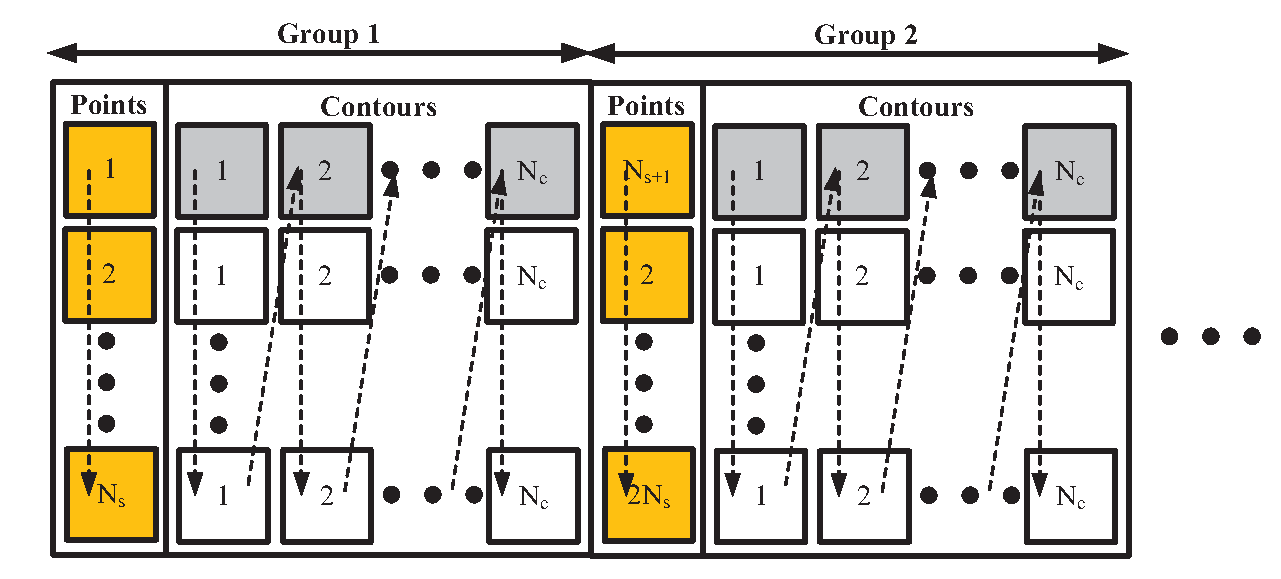
\includegraphics[width=0.7\textwidth]{3_precision/figures/stream}
\end{center}
\caption{Data structure: 
$N_S$ points are processed in a group. 
Each point of a group is iterated for $N_C$ times.
Data are streamed in an order as indicated by the arrows.}
\label{fig:precision_stream}
\end{figure}

\subsection{System Architecture}
Figure~\ref{fig:precision_arch} shows our proposed system architecture which consists of three major components.

\begin{figure}[t!]
\begin{center}
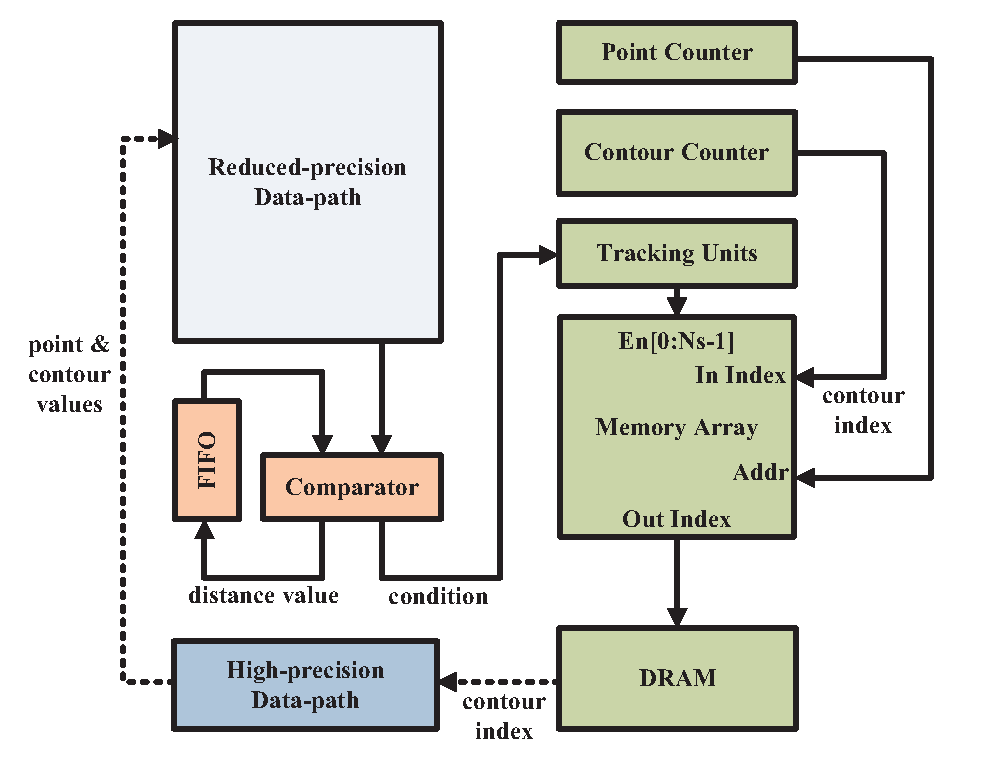
\includegraphics[width=0.7\textwidth]{3_precision/figures/arch}
\end{center}
\caption{System architecture:
Solid lines represent communication on the FPGA board while dotted lines represent the bus connecting the reduced precision data-path on FPGA to the high precision data-path on CPU.
}
\label{fig:precision_arch}
\end{figure}

\noindent \textbf{Data-paths:}
As mentioned in Section~\ref{sec:precision_optimisation}, we employ reduced precision on \gls{fpga} to compute the deviations.
The high precision data-path on \gls{cpu} re-computes the deviations which are not sufficiently accurate,
and then it calculates the penetration depth based on the minimum deviation.
The reduced precision and high precision data-paths are interfaced by a comparator and a memory architecture as described below.

\noindent \textbf{Comparator:}
The comparator compares the values of two point-segment distances and determines which one is smaller.
Consider a group of $N_{S}$ points (i.e. $\boldsymbol{x_1}$, $\boldsymbol{x_2}$, ..., $\boldsymbol{x_{N_S}}$) being processed together in the pipeline, we use a FIFO of length $N_{S}$ where
each slot of the FIFO stores the latest minimum deviation corresponding to a point.
Since the point-segment distances are calculated in reduced precision, according to Section~\ref{sec:precision_mixed_precision}, 
either one of the three conditions happens:
(A) The distance from the data-path is smaller; 
(B) The distance stored in the FIFO is smaller; 
(C) The difference between the two distances is too small, so re-computation in high precision is necessary.

\noindent \textbf{Memory Architecture:}
The purpose of the memory architecture is to store the contours that require re-computation.
We design a memory array as shown in Figure~\ref{fig:memory}.
There are $N_S$ rows, each of which corresponds to the computation of one point which is addressed by a \textit{point counter}.
Each row consists of $N_C$ elements and it serves as a buffer for contours that may need re-computation.
$N_C$ elements are needed as in the worst case all the contours have to be re-computed.
Instead of storing the contours in three-dimensional coordinate, we store their indices so as to save memory space.
The indices are counted by a \textit{contour counter}.
There are $N_S$ \textit{tracking units}, each for one row, to keep track of the latest elements where the indices should be written.

To understand the mechanism of memory architecture, consider the example in Figure~\ref{fig:memory1}.
First, the deviation in distance of \textit{point 1} is being calculated.
If the comparator indicates \emph{condition A}, the value from the reduced precision data-path is the smallest, and all previous values stored in that row will be cleared.
Second, the index corresponding to the new value is written to \textit{element 1} of \textit{row 1}.
Third, \textit{tracking unit 1} is updated to point to that element.
If \emph{condition B} is indicated, the minimum value is already stored in the memory and no update is required.
Consider another example in Figure~\ref{fig:memory2} where the calculation of \textit{point $N_S$} indicates \emph{condition C}. 
Both the indices in the memory and from the data-path should be stored.
Thus, a contour index is written to the next element and \textit{tracking unit $N_S$} advances one element further.

After a group of points are processed, the contour indices stored in the memory array are transferred to the \gls{dram} on the \gls{fpga} board.
The data on \gls{dram} will be accessed by the high precision data-path.
To fully utilise the memory bandwidth, only non-empty memory columns are transferred in burst to the \gls{dram}.

\setcounter{subfigure}{0}
\begin{figure}[t!]
\centering
\subfigure[Condition A: the value from the reduced precision data-path is the smallest, \textit{tracking unit 1} points to the \textit{element 1} of \textit{row 1}.
Previous vales stored in \textit{row 1} are cleared.]
{
	\includegraphics[width=0.6\textwidth]{3_precision/figures/test1}
	\label{fig:memory1}
}
\subfigure[Condition C: both the value in the memory and the index from the data-path should be stored. A contour index is written to the next element and \textit{tracking unit $N_S$} advances one element further.]
{
	\includegraphics[width=0.6\textwidth]{3_precision/figures/test2}
	\label{fig:memory2}
}
\caption{Memory array stores contour indices for re-computation.}
\label{fig:memory}
\end{figure}

\subsection{Performance Estimation}
\label{sec:precision_model}

We derive a performance model to make the most effective use of the \gls{fpga}'s resources and to address real-time requirements.
The results will be presented in Section~\ref{sec:precision_parallelism} and~\ref{sec:precision_recompute}.
The total computation time $T_{comp}$ is affected by the time spent on three parts:
(1) the reduced precision data-path on \gls{fpga},
(2) the high precision data-path on \gls{cpu},
(3) the data transfer through the bus connecting the \gls{cpu} to \gls{fpga}.
Equation~\ref{eqt:fM} shows the three parts respectively:

\begin{equation}
\begin{aligned}
T_{comp,p_L} = T_{p_L} + T_{p_H} + T_{tran} \mbox{,} \\
TH_{comp,p_L} = \frac{1}{T_{comp,p_L}} \mbox{,}
\end{aligned}
\label{eqt:fM}
\end{equation}

where $T_{p_L}$, $T_{p_H}$ and $T_{tran}$ represent the time spent on (1), (2) and (3) respectively.

The computation time of \gls{fpga}, $T_{p_L}$, is shown in Equation~\ref{eqt:fL}:

\begin{equation}
\begin{aligned}
T_{p_L} = \frac{N_P \cdot (N_C+L_{output})}{freq_{p_L} \cdot N_{p_L}} + L_{p_L} \mbox{,}
\end{aligned}
\label{eqt:fL}
\end{equation}

where $N_P$ is the number of points, $N_C$ is the number of contours,
$L_{p_L}$ is the length of the data-path but this term is usually negligible when compared with the amount of data being processed.
Each point needs $L_{output}$ cycles to output indices on the memory array to \gls{dram}.

$L_{output}$ is affected by the bit-width available between the \gls{fpga} and the \gls{dram} and their relations are shown in Equation~\ref{eqt:output}:

\begin{equation}
\begin{aligned}
L_{output} = \frac{N_C}{N_{output}} \mbox{ , } \quad
N_{output} = \frac{W_{DRAM}}{W_{idx} \cdot N_{p_L}} \mbox{.}
\end{aligned}
\label{eqt:output}
\end{equation}

The computation time of \gls{cpu}, $T_{p_H}$, is related to the amount of data and the ratio of re-computation:

\begin{equation}
\begin{aligned}
T_{p_H} = \alpha \cdot R \cdot N_P \cdot N_C \mbox{.}
\end{aligned}
\label{eqt:fH}
\end{equation}

The data transfer time from the \gls{dram} to \gls{cpu}, $T_{tran}$, is judged by the amount of data, the ratio of re-computation, $R$,and the bandwidth of the bus connecting the \gls{cpu} to \gls{fpga}, $BW_{bus}$:

\begin{equation}
\begin{aligned}
T_{tran} = \frac{R \cdot N_P \cdot N_C \cdot W_{idx}}{BW_{bus}} \mbox{.}
\end{aligned}
\label{eqt:tran}
\end{equation}

With the model, designer can ensure that the system parameters (Table~\ref{tab:model}) do not cause the system to fail real-time application's deadline.

\begin{table}[t!]
	\begin{spacing}{1.0}
	\caption{Parameters of the performance model.}
	\label{tab:model}
	\centering
	\smallskip
	\begin{tabular}{l|l}
			\hline
			$N_P$			& Num. of points \\
			$N_C$			& Num. of contours \\
			$N_{p_L}$ 		& Num. of reduced precision data-path \\
			$N_{p_H}$ 		& Num. of high precision data-path \\
			$L_{p_L}$			& Length of the data-path \\
			$N_{output}$ 	& Num. of outputs per data-path per cycle \\
			$L_{output}$ 	& Num. of output cycles \\
			$L_{cmp}$			& Latency of a comparison operation \\
			$R$ 			& Ratio of re-computation \\
			$W_{DRAM}$ 		& Bit-width of \gls{fpga}-\gls{dram} connection \\
			$W_{idx}$ 		& Bit-width of one contour index \\
			$freq_{p_L}$  	& Clk. freq. of reduced precision data-path \\
			$\alpha$ 		& Empirical constant of \gls{cpu} speed \\
			$BW_{bus}$ 	& Bandwidth of the bus connecting the \gls{cpu} to \gls{fpga} \\
			\hline
		\end{tabular}
	\end{spacing}
\end{table}

%For full-precision, shown in Equation~\ref{eqt:fH}.
%Reduced-precision data-path uses fewer resources than the high precision, so $N_{p_H}$ is smaller than $N_{p_L}$.
%$freq_{p_L}$ is also higher than $freq_{p_H}$.
%To have benefit, speed up $\frac{T_{Mixed}}{T_{p_H}}$ should be greater than 1.
%
%\begin{equation}
%\begin{aligned}
%T_{p_H} = \frac{N_P \cdot (N_C)}{freq_{p_H} \cdot N_{p_H}}
%\end{aligned}
%\label{eqt:fH}
%\end{equation}


%%%%%%%%%%%%%%%%%%%%%%%%%%%%%%%%%%%%%%%%%%%%%%%%%%%%%%%%%%%%%%%%%%%%%%%%%%%%%%%%%%%%%%%%%%%%%%%%%%%%%%%%%%%%%%%%%%%%%%%%%%%%%%%%%%%%%%%%%%%%%%%%
\section{Experimental Evaluation}
\label{sec:precision_evaluation}

\subsection{General Settings}
We use the MPC-C500 reconfigurable system from Maxeler Technologies for our evaluation.
The system has four MAX3 cards, each of which has a Virtex-6 XC6VSX475T \gls{fpga} with 476,100 logic cells and 2,016 \glspl{dsp}.
The cards are connected to two Intel Xeon X5650 \gls{cpu}s and each card communicates with the \gls{cpu}s via a PCI Express gen2 x8 link. 
The \gls{cpu}s have 12 physical cores and are clocked at 2.66 GHz.
We develop the \gls{fpga} kernels using MaxCompiler which adopts a streaming programming model supporting customisable floating-point data formats.

We also build a \gls{cpu}-based system by implementing the \gls{pq} formulation on a platform with two Intel Xeon X5650 \gls{cpu}s running at 2.66 GHz.
The code is written in C++ and compiled by Intel C compiler with the highest optimisation.
OpenMP library is used to parallelise the program for multiple cores.
IEEE double precision floating point numbers are used.

For the \gls{gpu}-based system, we use an NVIDIA Tesla C2070 \gls{gpu} which has 448 cores running at 1.15 GHz.

Our \gls{pq} implementation supports 100 contours and we set an update rate of 1~kHz as the real-time requirement.

\subsection{Parallelism versus Precision}
\label{sec:precision_parallelism}

Figure~\ref{fig:exectime} shows the overall computation time ($T_{Comp}$)
and the degree of parallelism of \gls{pq} versus different number of mantissa bits.
Please note that all different configurations of mantissa bits have the same output accuracy.
The data set includes 73k points and 100 contours.
The computation times are obtained using our analytical model in Section~\ref{sec:precision_model} and they are verified experimentally using the implementation.
The degree of parallelism is obtained by filling the \gls{fpga} with data-paths until the logic cell utilisation exceeds 80\% after the placement and routing process.
The degree of parallelism is the highest when we start with four mantissa bits.
Using more mantissa bits decreases the parallelism as well as the ratio of re-computation, therefore $T_{p_L}$ increases but $T_{p_H}$ decreases.
As shown by the dotted line in the figure, a minimum computation time is achieved when 10 mantissa bits are used.
Note that when the number of mantissa bits is more than~36, only one data-path can be mapped onto the \gls{fpga}.
In such cases, we can implement the data-path in double precision directly which does not require any re-computation on \gls{cpu}.
This is indicated by the last data points of both curves.

\begin{figure}[ht]
\begin{center}
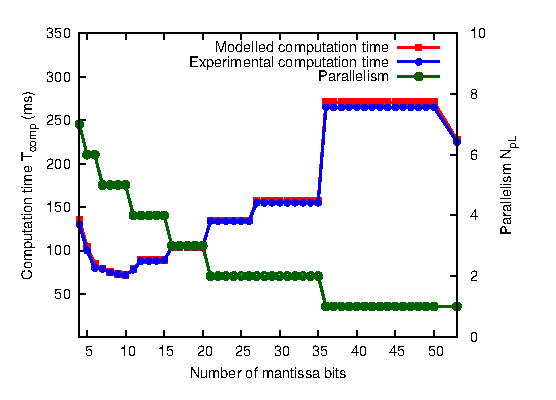
\includegraphics[width=0.7\textwidth]{3_precision/figures/fig_exectime}
\end{center}
\caption[Computation time and the level of parallelism versus different number of mantissa bits.]{Computation time (dotted line) and the level of parallelism (solid line) versus different number of mantissa bits.}
\label{fig:exectime}
\end{figure}

\subsection{Ratio of Re-computation versus Precision}
\label{sec:precision_recompute}
The dotted line in Figure~\ref{fig:recompute} shows the ratio of re-computation versus the number of mantissa bits.
The results are obtained from a software version of \gls{pq} implementation with precisions adjusted using MPFR library~\cite{fousse07}.
For each point, 100 computations of deviation in distance are required.
The ratio of re-computation drops exponentially as the number of mantissa bits increases.
From the performance perspective, to the left the ratio of re-computation is too high, to the right the decrease of re-computation cannot offset the impact brought by the decrease in parallelism.
When the number of mantissa bits is four, in average 2.66 out of 100 computations need to be re-computed using high precision, i.e. the ratio of re-computation is 2.66\%.
When the number of mantissa bits is greater then 15, the ratio of re-computation drops to 1\% which is the minimum value as only one out of 100 values is re-computed.
The last data points of both curves indicate the situation when double precision is used on the \gls{fpga} and no re-computation is necessary.

The solid line in Figure~\ref{fig:recompute} shows the number of point processed in 1~ms versus the number of mantissa bits.
The application has a real-time update requirement of 1~kHz so the results are updated every 1~ms.
The number of required points is based on the user specification of the model resolution in three-dimensional space.
When the number of mantissa bits is 10, the maximum number of points can be processed.
It is because the throughput is the highest by balancing the ratio of re-computation and the degree of parallelism.
Since more points can be processed in real-time, we can handle a more complex robot model with a finer resolution.

\begin{figure}[ht]
\begin{center}
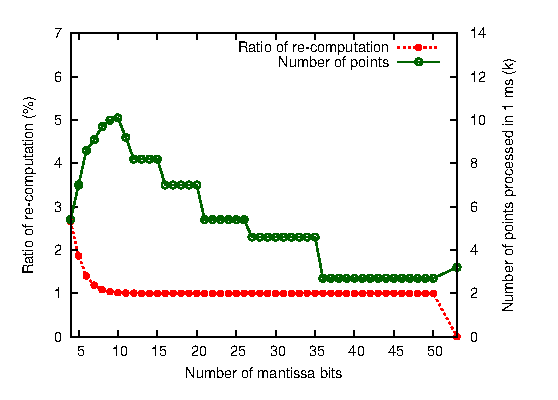
\includegraphics[width=0.7\textwidth]{3_precision/figures/fig_recompute}
\end{center}
\caption[Ratio of re-computation and the number of points processed in 1 ms versus different number of mantissa bits.]{Ratio of re-computation (dotted line) and 
the number of points processed in 1 ms (solid line) versus different number of mantissa bits.}
\label{fig:recompute}
\end{figure}

\subsection{Comparison: CPU, GPU and Reconfigurable System}
Table~\ref{tab:performance} compares the performance of \gls{pq} running on \gls{cpu}, \gls{gpu} and \gls{fpga} in double precision arithmetic, 
and our proposed reconfigurable system with \gls{cpu}s and \gls{fpga}s.

%For the \gls{fpga}-based implementation, the double-precision design is too large to fit into the \gls{fpga} chip.
%Thus, we assume the implementation is realised on a larger \gls{fpga} and the results are obtained by the performance model in Section~\ref{sec:implementation}.

In 1~ms, our proposed system is able to process 58 times more points than a 12-core \gls{cpu} system, and 9 times more points than a \gls{gpu} system.
Without any optimisation, we can only implement one double precision data-path on an \gls{fpga}.
Our proposed approach can support five reduced precision data-paths to be implemented in parallel on one chip, i.e.~20 data-paths in total on the 4-\gls{fpga} system.
The clock frequency is also higher because reduced precision simplifies routing of signals.
The performance gain over a double precision \gls{fpga} implementation is over 3 times.

%\newcolumntype{g}{>{\columncolor{Gray}}c}
\begin{table}[t!]
	\begin{spacing}{1.0}
	\caption{Comparison of PQ computation in 1 ms using CPU-based system (CPU), GPU-based system (GPU), double precision FPGA-based reconfigurable system (RS DP) and FPGA+CPU reconfigurable system with reduced precision (RS RP).}
	\label{tab:performance}
	\centering
	\smallskip
	\begin{threeparttable}
		\begin{tabular}{l|c|c|c|g}
			\hline
			  							& \gls{cpu} 		& \gls{gpu}  	& RS DP 		& RS RP \\
			\hline
			Clock freq. (MHz) 			& 2,660 	& 1,150 			& 80 			& 130 \& 2,660 \tnote{a}  \\
			Num. of cores				& 12		& 448				& 4 			& 20 \\
			\hline
			Num. of mantissa bits		& 53		& 53				& 53			& 10 \& 53 \tnote{b} \\
			Num. of $p_L$ eval. (k)		& 0 		& 0 				& 0 			& 1009.4 \\
			Num. of $p_H$ eval. (k)		& 173 		& 106 				& 320			& 10.1 \\
			Num. of total eval. (k)		& 173 		& 106 				& 320			& 1019.5 \\
			Eval. in $p_H$ (\%) 		& 100		& 100				& 100 			& 1 \\
			\hline
			Num. of points in 1 ms		& 173		& 1,064				& 3,200 		& 10,094 \\
			Normalised speedup 			& 1x 		& 6.15x 				& 18.5x 		& 58.35x \\
			Reduced precision gain 		& -  		& -  				& 1x 			& 3.15x  \\
			\hline
		\end{tabular}
		\begin{tablenotes}		
		\item[a] \gls{fpga} and \gls{cpu} clock frequencies.
		\item[b] Reduced precision and high precision.
		\end{tablenotes}
	\end{threeparttable}
	\end{spacing}
\end{table}

Figure~\ref{fig:scalability} shows the computation time for a \gls{pq} update against the number of points.
The black solid line indicates the real-time bound of 1~ms.
In the \gls{cpu}-based system, even with the fastest configuration (12 cores), only 173 points can be processed in real-time.
Meanwhile, the performance of our proposed 1-\gls{fpga} reconfigurable system is on-par with a 4-\gls{fpga} reconfigurable system in double precision.
Our proposed 4-\gls{fpga}s system can process 10,094 points within the 1~ms interval.

\begin{figure}[ht]
\begin{center}
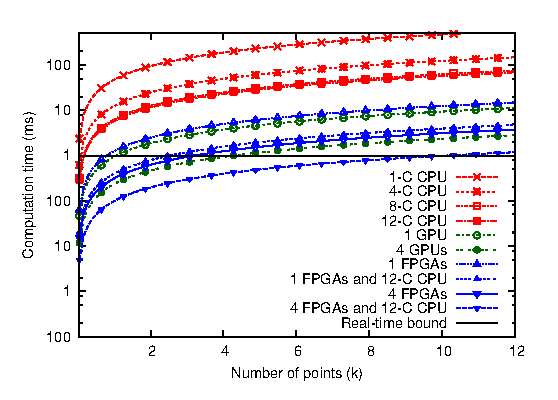
\includegraphics[width=0.7\textwidth]{3_precision/figures/fig_scalability}
\end{center}
\caption{Computation time for a PQ update with 100 contours versus the number of points.}
\label{fig:scalability}
\end{figure}

%%%%%%%%%%%%%%%%%%%%%%%%%%%%%%%%%%%%%%%%%%%%%%%%%%%%%%%%%%%%%%%%%%%%%%%%%%%%%%%%%%%%%%%%%%%%%%%%%%%%%%%%%%%%%%%%%%%%%%%%%%%%%%%%%%%%%%%%%%%%%%%%
\section{Summary}
\label{sec:precision_summary}

This chapter presents a reconfigurable computing solution to proximity query computation.
To the best of our knowledge, this is the first application of \glspl{fpga} to this problem.
%our approach is the first to apply \gls{fpga}s to this problem.

We transform the algorithm to enable pipelining and apply reduced precision methodology to maximise parallelism.
Run-time reconfiguration is employed to optimise precision automatically.
We then map the optimised algorithm to a reconfigurable system with four Virtex-6 \gls{fpga}s and 12 \gls{cpu} cores.
Our proposed reconfigurable system achieves 478 times speedup over a single-core \gls{cpu}, 58 times speedup over a 12-core \gls{cpu} system, 9 times speedup over a \gls{gpu},
and 3 times speedup over an \gls{fpga} implementation in double precision.
Since more points can be processed in real-time, we can handle a more complex robot model with a finer resolution.
